\documentclass{article}

\usepackage{graphicx}
\usepackage{tikz}
\usepackage{tikzsymbols}
\usetikzlibrary{calc,patterns,shapes.geometric}
\pagestyle{empty}
\usepackage[margin=0pt]{geometry}
\geometry{papersize={14in,12in}}

\def\centerarc[#1](#2)(#3:#4:#5){\draw[#1] ($(#2)+({#5*cos(#3)},{#5*sin(#3)})$) arc (#3:#4:#5);}

\begin{document}
	\begin{figure}
		\centering
		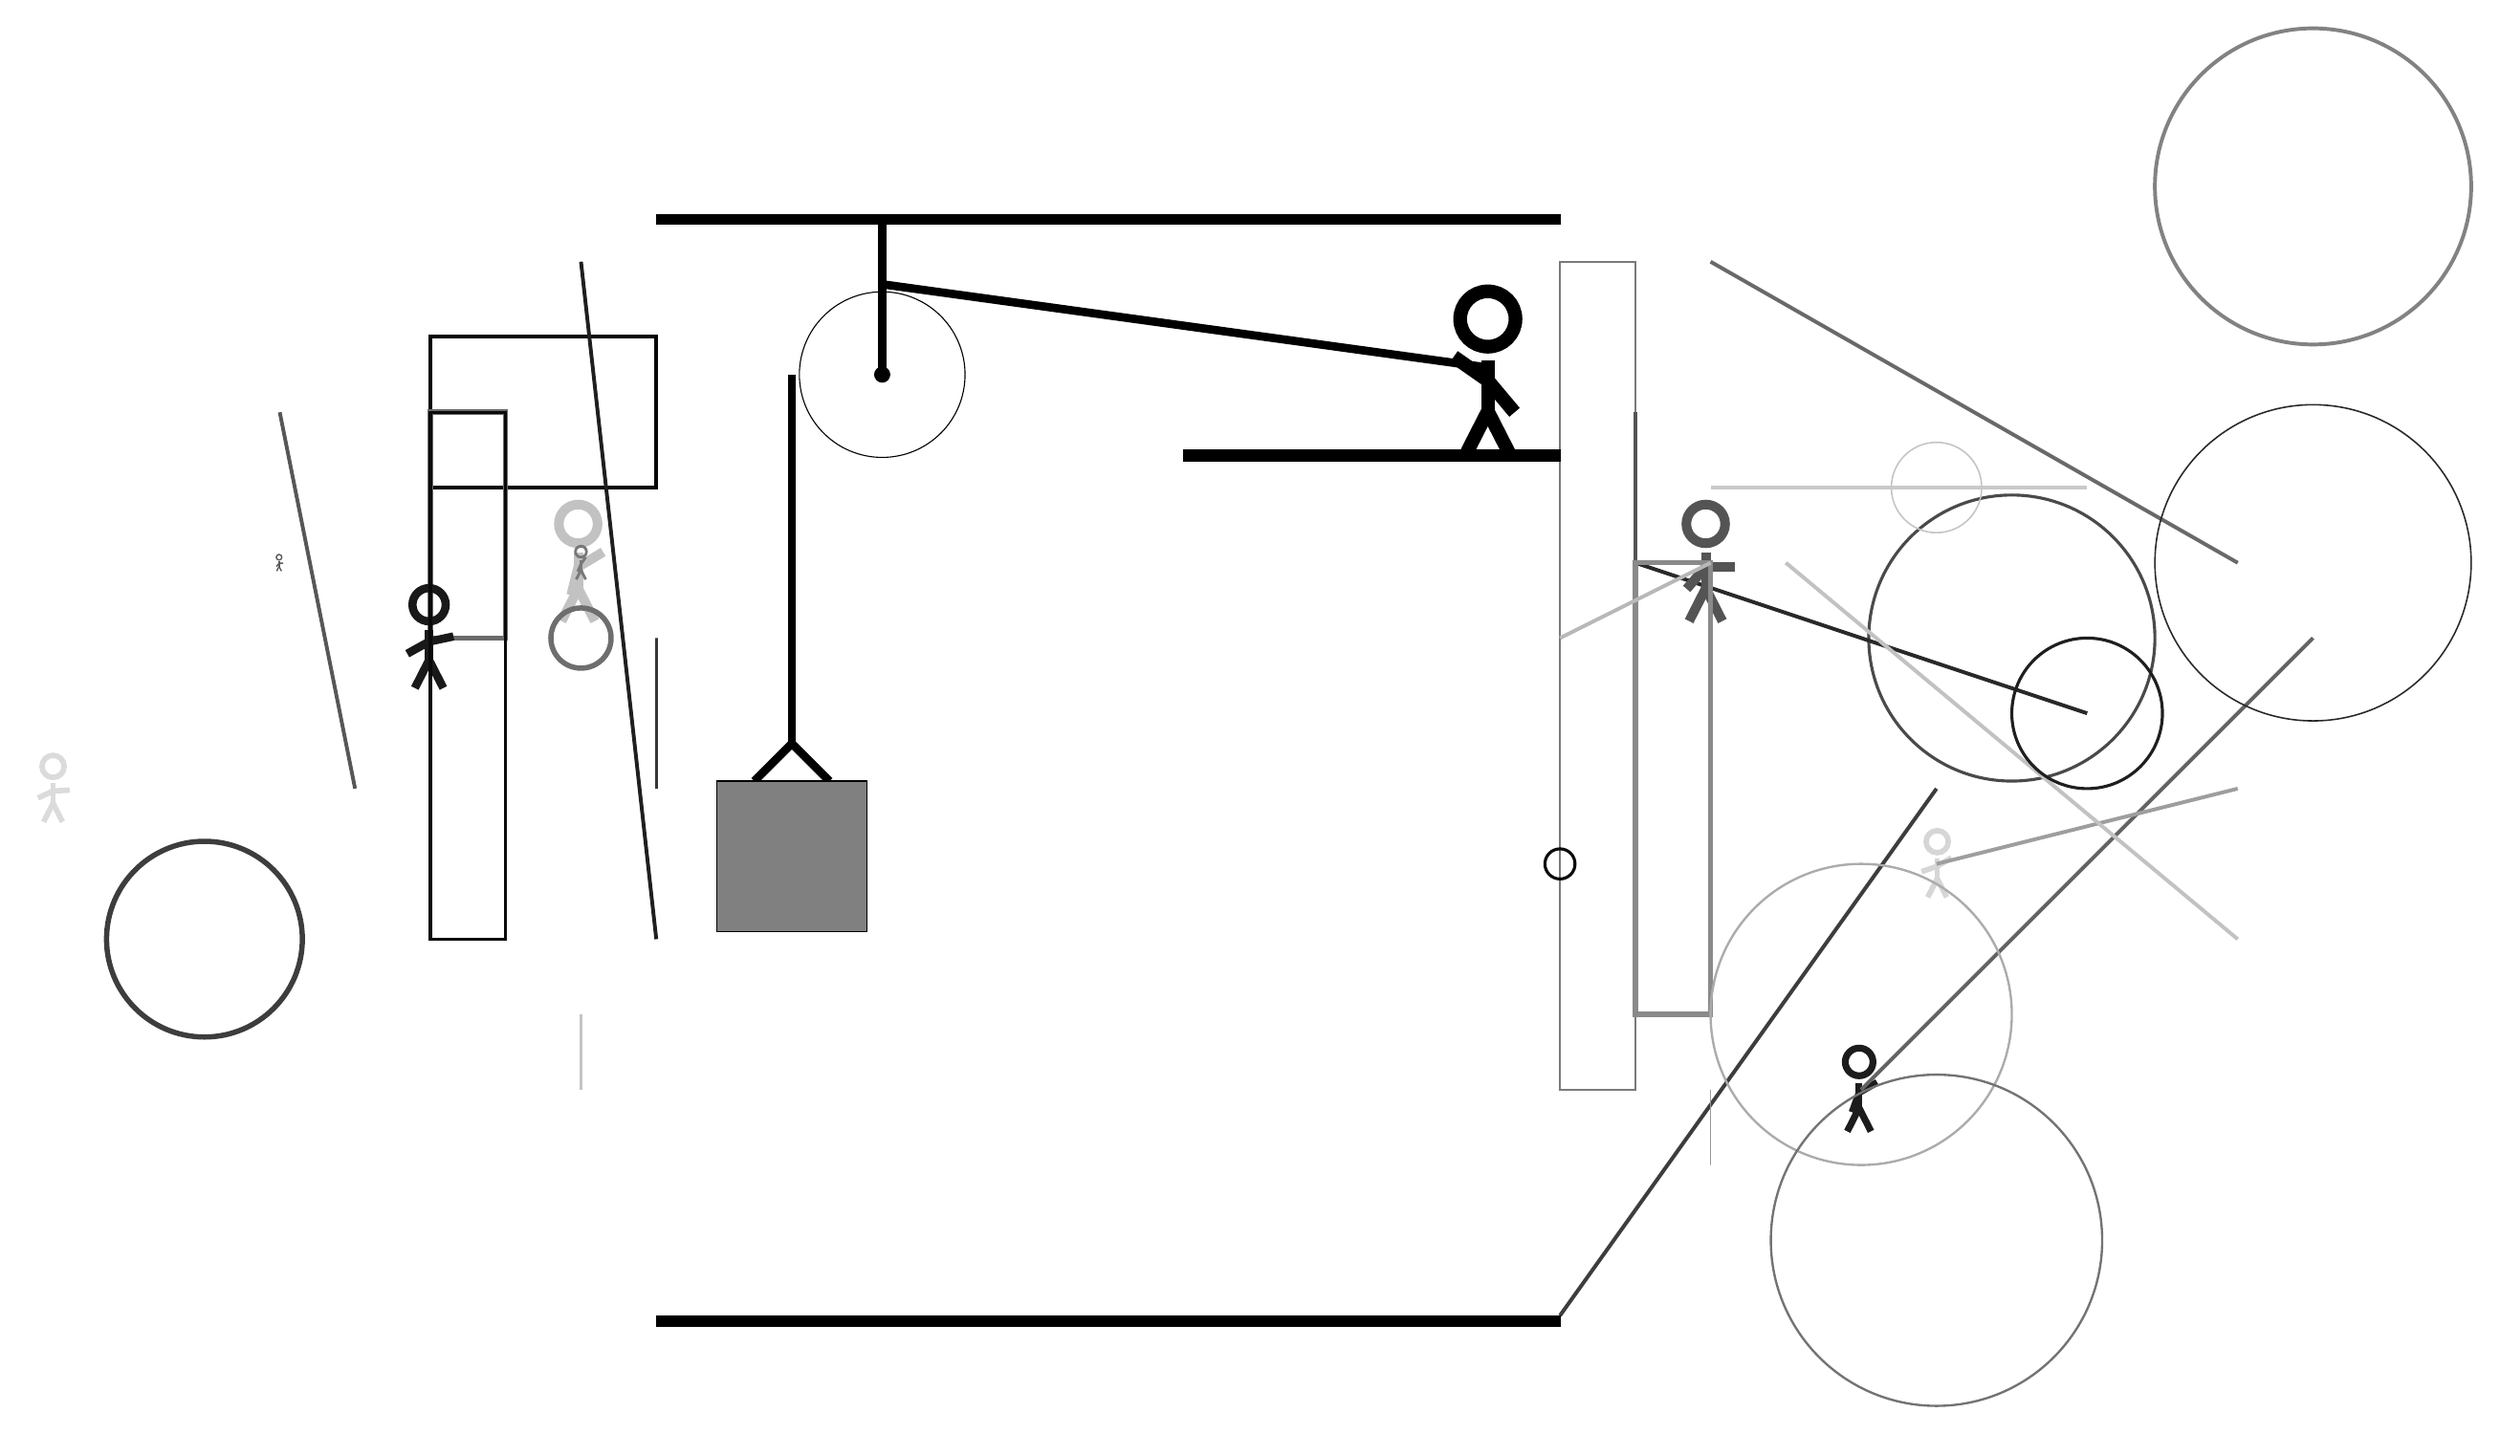
\begin{tikzpicture}
			%%%%% START %%%%%
			
			\draw[fill=black] (-2, 11.5) rectangle (10, 11.625);
			
			\draw (1, 9.5) circle (1.1);
			\draw[fill=black] (1, 9.5) circle (0.1);
			\draw[line width=1.1mm] (1, 11.5) -- (1, 9.5);
			
			\draw[line width=1.1mm](-0.7, 4.1) --  (-0.2, 4.6) -- (0.3, 4.1);
			\draw[fill=black!50] (-1.2, 4.1) rectangle (0.8, 2.1);
			
			\draw[line width=1.1mm](-0.2, 9.5) -- (-0.2, 4.6);
			\centerarc[line width=1.1mm](1, 9.5)(90:180:1.2000000000000002)
			\draw[line width=1.1mm](1, 10.7) -- (9, 9.6);
			
			\node[line width=0.7mm, color=black!89] at (14, 0) {\Strichmaxerl[5][70][30]};
			
			\node[line width=0.2mm, color=black!14] at (-10, 4) {\Strichmaxerl[4][25][3]};
			\draw[line width=0.5mm, color=black!98] (-2, 10) rectangle (-5, 8);
			\draw[line width=0.3mm, color=black!52] (11, 11) rectangle (10, 0);
			
			\draw [line width=0.4mm, color=black!71](16, 6) circle (1.9);
			
			\draw [line width=0.5mm, color=black!16](13, 11) circle (0.0);
			
			\draw[line width=0.5mm, color=black!76](15, 4) -- (10, -3);
			
			\draw[line width=0.5mm, color=black!84](11, 7) -- (17, 5);
			\draw[line width=0.4mm, color=black!79] (-2, 6) rectangle (-2, 4);
			\draw[line width=0.5mm, color=black!23] (-3, 0) rectangle (-3, 1);
			
			\draw[line width=0.5mm, color=black!61](14, 0) -- (20, 6);
			\node[line width=0.5mm, color=black!67] at (12, 7) {\Strichmaxerl[7][49][0]};
			\draw[line width=0.5mm, color=black!59](12, 11) -- (19, 7);
			
			\draw [line width=0.7mm, color=black!76](-8, 2) circle (1.3);
			\draw[line width=0.5mm, color=black!88](-3, 11) -- (-2, 2);
			\draw[line width=0.7mm, color=black!58] (-4, 9) rectangle (-5, 6);
			
			\draw[line width=0.5mm, color=black!66](-7, 9) -- (-6, 4);
			\draw[line width=0.2mm, color=black!40] (12, -1) rectangle (12, 0);
			\node[line width=0.3mm, color=black!16] at (15, 3) {\Strichmaxerl[4][19][31]};
			\node[line width=0.2mm, color=black!24] at (-3, 7) {\Strichmaxerl[7][76][31]};
			\draw[line width=0.5mm, color=black!38](15, 3) -- (19, 4);
			\draw [line width=0.2mm, color=black!84](20, 7) circle (2.1);
			
			\draw [line width=0.5mm, color=black!49](20, 12) circle (2.1);
			\draw[line width=0.5mm, color=black!24](13, 7) -- (19, 2);
			\draw[line width=0.5mm, color=black!67] (11, 7) rectangle (11, 9);
			
			\draw[line width=0.7mm, color=black!46] (12, 1) rectangle (11, 7);
			\draw [line width=0.4mm, color=black!88](17, 5) circle (1.0);
			\node[line width=0.2mm, color=black!64] at (-7, 7) {\Strichmaxerl[1][49][4]};
			
			\node[line width=0.6mm, color=black!53] at (-3, 7) {\Strichmaxerl[2][67][55]};
			\node[line width=0.2mm, color=black!90] at (-5, 6) {\Strichmaxerl[6][29][12]};
			\draw [line width=0.4mm, color=black!96](10, 3) circle (0.2);
			
			\draw [line width=0.2mm, color=black!23](15, 8) circle (0.6);
			\draw[line width=0.5mm, color=black!28](12, 7) -- (10, 6);
			\draw[line width=0.4mm, color=black!96] (-4, 9) rectangle (-5, 2);
			\draw [line width=0.3mm, color=black!33](14, 1) circle (2.0);
			\draw [line width=0.7mm, color=black!57](-3, 6) circle (0.4);
			\draw [line width=0.3mm, color=black!55](15, -2) circle (2.2);
			
			\draw[line width=0.5mm, color=black!21](12, 8) -- (17, 8);
			
			\node at (9, 9.5) {\Strichmaxerl[10][-35][-50]};
			\draw[fill=black] (5, 8.5) rectangle (10, 8.35);
			
			\draw[fill=black] (-2, -3) rectangle (10, -3.15);
			
			%%%%% END %%%%%
		\end{tikzpicture}
	\end{figure}	
\end{document}